\chapter{Simulácia a porovnanie}
\label{part:Simulacie}
V tejto kapitole si overíme teóriu, ktorej sme sa venovali v predošlých častiach. Budeme využívať distribuované MPC na riadenie diskrétneho systému. Nebudeme pracovať so simuláciou v reálnom čase na kontinuálnom systéme, a to z dôvodu, že táto práca je zameraná čisto na zrýchlenie výpočtového času MPC. Našou úlohou bude overiť, či distribuovanie prediktívneho regulátora na jednotlivé kroky predikčného horizontu pomôže znížiť jeho výpočtový čas. Ako prvé vykonáme simuláciu na lineárnom modeli, ktorý bude reprezentovať pohyb hmotného bodu v priestore. Po overení teórie na linearnom systéme môžeme prejsť k nelineárnemu modelu. Budeme pracovať s modelom DC motora a to je zariadenie, ktoré má veľmi rýchlu dynamiku. Nedá sa jednoducho riadiť nelineárnym regulátorom vzhľadom na to, že jeho perióda vzorkovania sa pohybuje v desiatkach milisekúnd.

\section{Pohyb hmotného bodu v priestore}
\label{sec:HB}
Majme hmotný bod, ktorý sa pohybuje v priestore a je opísaný nasledovnými diskrétnymi rovnicami s periódou vzorkovania $Ts = 1s$.
\label{math:model_HB}
\begin{align}
&x_{k+1}^{1} = x_{k}^{1} + x_{k}^{2} + u_{k}\\
&x_{k+1}^{2} = x_{k}^{2} + 0,5u_{k}
\end{align}
Prvý stav $x_{1}$ predstavuje polohu a druhý stav $x_{2}$ predstavuje rýchlosť hmotného bodu. Pomocou týchto rovníc si môžeme zostrojiť maticu stavov $A$ a maticu vstupov $B$
\begin{align}
A = \begin{bmatrix}
1 &1\\
0 &1
\end{bmatrix},
B= \begin{bmatrix}
1\\
0,5
\end{bmatrix}
\end{align}
a následne ich dosadíme do lineárneho stavového opisu systému.
\begin{align}
& x_{k+1} = Ax_{k}+Bu_{k}
\end{align}
Takto zostrojený model systému využijeme pri návrhu lineárneho MPC s predikčným horizontom $N = 5$, podľa teórie uvedenej v kapitole \hyperref[subse:MPC]{Formulácia MPC (2.1.1)}. Následne si rozdistribuujeme a upravíme takto navrhnuté MPC na $N = 5$ predikčných horizontov podľa postupu, ktorý sme si uviedli v kapitole \hyperref[subse:Lin_MPC_ADMM]{Lineárne prediktívne riadenie pomocou ADMM (2.4.1)}. Ako kritériá pre zastavenie \hyperref[subse:ADMM2]{iterácií v ADMM} sme zvolili presnosť hľadaných počiatočných stavov $\norm{\tilde{H}_{1}U_{k-1}^{i} + \tilde{H}_{2}U_{k} - \tilde{A}U_{k-1}^{i}} < \epsilon,\hspace{0.5cm} k=1,\dots,N-1$ (veľkosť duálnej funkcie) a taktiež veľkosť zmeny predikovaných akčných zásahov $\norm{U(1)_{k}^{i-1}-U(1)_{k}^{i}} < \epsilon,\hspace{0.5cm} k=0,\dots,N-1$, kde $\epsilon = 1\mathrm{e}{-5}$. Akonáhle sa jedna z týchto podmienok splní, môžeme prehlásiť, že sme našli optimálne akčné zásahy. Rovnako, ako v obyčajnom MPC, zoberieme prvý akčný zásah $u_{0}$, aplikujeme ho a ostatné zahodíme. Tento postup opakujeme, pokiaľ neskonvergujeme do optima (odchýlka stavov rovná nule, alebo sa dostaneme na žiadanú hodnotu).

Vytvorili sme jednoduchú simuláciu na modeli uvedenom v \hyperref[math:model_HB]{rovniciach (3.1,3.2)}, aby sme boli schopní porovnať normálne MPC s decentralizovaným MPC.
\begin{figure}[H]
	\centering
	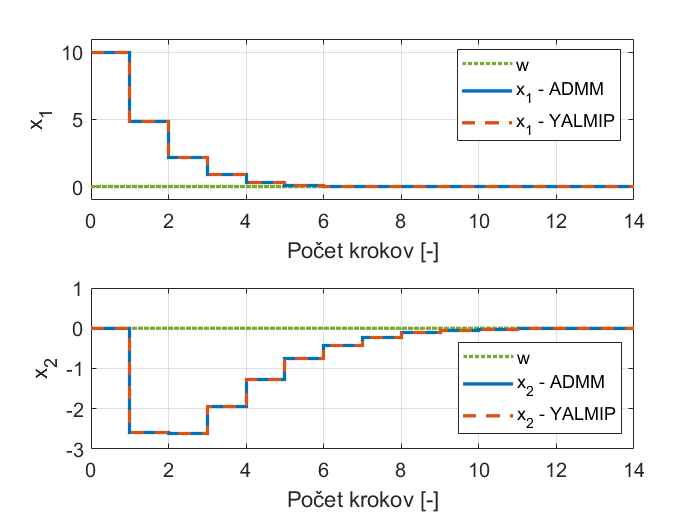
\includegraphics[width=13cm,height=10cm]{images/Hmotny_bod/Priebeh_riadenia}
	\caption{Priebeh riadenia pre lineárny systém}
	\label{fig1: PRLS}
\end{figure}
Ako môžeme vidieť na (Obr. 3.1), v oboch prípadoch sa nám podarilo dosiahnuť žiadanú veličinu (nulovú odchýlku stavov) a priebeh riadenia ja totožný pri oboch metódach.
\begin{figure}[H]
	\centering
	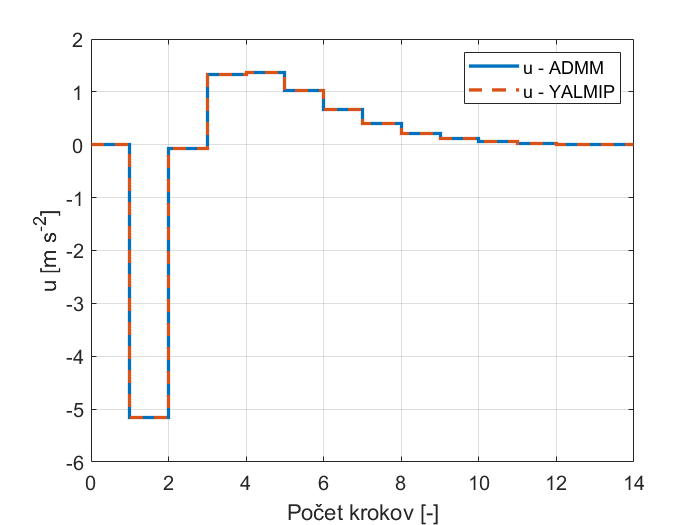
\includegraphics[width=13cm,height=10cm]{images/Hmotny_bod/Akcne_zasahy}
	\caption{Vývoj akčných zásahov}
	\label{fig2:AZLS}
\end{figure}
Rovnako ako stavy, tak aj akčné zásahy, sú totožné pri oboch metódach, čo môžeme vidieť na (Obr. 3.2).
\newpage
\begin{figure}[H]
	\centering
	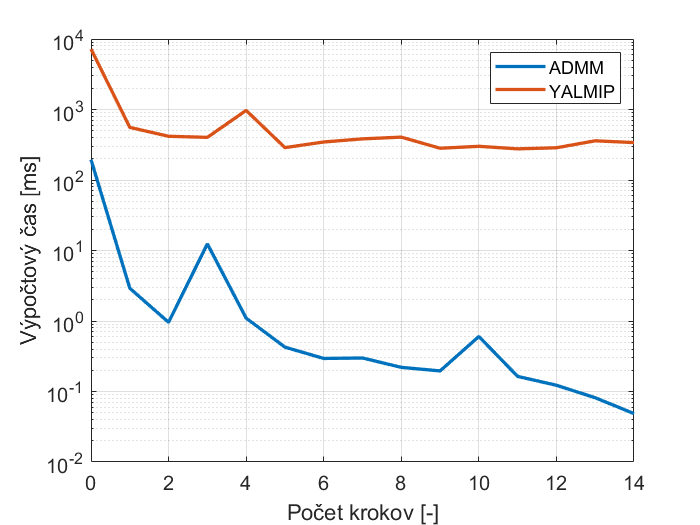
\includegraphics[width=13cm,height=10cm]{images/Hmotny_bod/Vypoctovy_cas}
	\caption{Porovnanie výpočtovej náročnosti MPC, medzi ADMM a YALMIP}
	\label{fig3: VNAA}
\end{figure}
Pre nás je najdôležitejší graf výpočtovej náročnosti (Obr. 3.3). Ako môžeme vidieť, podarilo sa nám dosiahnuť značné zlepšenie oproti analytickému riešiteľu z toolboxu YALMIP. Zatiaľ čo inicializačný čas pre ADMM bol okolo 100ms, najrýchlejšie riešenie pomocou YALMIP sa pohybovalo vyššie ako 100ms. Z tohoto porovnania vyplýva, že ADMM metóda je lepšia pre systémy s rýchlou dynamikou ($T_{s} \geq 1s $), ak sú opísané lineárnym matematickým modelom. 
\newpage


\section{Optimálne zastavenie DC motora}

DC motor je často využívaným zariadením v priemysle, ale aj v bežnom živote. Môže nadobúdať rôzne veľkosti a formy a jeho účelom je meniť elektrickú energiu na energiu mechanickú. Čo je pre nás dôležité, pracuje pod veľmi malou periódou vzorkovania. Je to teda systém s veľmi rýchlou dynamikou a nedá sa jednoducho riadiť pomocou nelineárneho MPC. 
\label{math:model_DC}
V tomto prípade budeme mať model systému opísaný nelineárnymi diferenciálnymi rovnicami, ktoré sú v nasledovnom tvare:
\begin{subequations}
	\begin{align}
	& \dot{x}^{(1)}(t) = - \frac{R}{L_{a}}x^{(1)}(t) - \frac{k_{m}}{L_{a}}u(t)x^{(2)}(t) + \frac{u_a}{L_a},\\
	& \dot{x}^{(2)}(t) = - \frac{B}{J}x^{(2)}(t) - \frac{k_{m}}{J}u(t)x^{(1)}(t) + \frac{\tau_l}{J},\\
	& y(t) = x^{(1)}(t),
	\end{align}
\end{subequations}
kde prvý stav $x^{(1)}$ predstavuje prúd rotora v $[A]$, druhý stav $x^{(2)}$ predstavuje uhlovú rýchlosť v $[rad/s]$ a vstupom $u$ je prúd statora udávaný v $[A]$. Naša sledovaná veličina bude uhlová rýchlosť (druhý stav)\cite{bib2}.
\begin{table}[h!]
	\centering
	\caption{Parametre DC motora \cite{bib2}}
	\label{tab.1: Parametre DC motora}
	\begin{tabular}{c c c}
		\hline
		\textbf{Značka} & \textbf{Hodnota} & \textbf{Veličina} \\ \hline
		$L_{a}$ & $0,314$ & $H$ \\ 
		$R_{a}$ & $12,345$ & $\Omega$ \\ 
		$k_{m}$ & $0,253$ & $N m A^{-2}$ \\ 
		$J$ & $0,00441$ & $N m s^{-2}$ \\ 
		$B_{a}$ & $ 0,00732$ & $N m s$ \\ 
		$\tau_l$ & $1,47$ & $N m$ \\
		$u_{a}$ & $60$ & $V$ \\ \hline
	\end{tabular}
\end{table}

Keďže máme model v kontinuálnej časovej oblasti, musíme si ho pretransformovať do diskrétnej podoby. Využijeme pri tom Eulerovu metódu, kde aproximujeme kontinuálny model diskrétnym podľa teórie, ktorú sme si uvideli v kapitole \hyperref[se:diskretizacia]{(2.2)}. Model systému po diskretizácií má nasledovnú podobu:
\begin{subequations}
\label{math:Dmodel_DC}
\begin{align}
& x_{k+1}^{(1)} = x^{(1)}_{k}+T_{s}\left(- \frac{R}{L_{a}}x^{(1)}_{k} - \frac{k_{m}}{L_{a}}u_{k}x^{(2)}_{k} + \frac{u_a}{L_a}\right),\\
& x_{k+1}^{(2)} = x^{(2)}_{k}+T_{s}\left(- \frac{B}{J}x^{(2)}_{k} - \frac{k_{m}}{J}u_{k}x^{(1)}_{k} + \frac{\tau_l}{J}\right),\\
& y(t) = x^{(1)}_{k},
\end{align}
\end{subequations}
kde $T_{s}$ je perióda vzorkovania , ktorú sme použili ako krok diskreditácie. Keďže sa jedná o veľmi rýchly systém, jeho perióda vzorkovania je veľmi malá, v našom prípade je to $T_{s} = 50ms$. Túto periódu musíme počas riadenia dodržiavať, ak chceme aby náš prediktívny regulátor bol stabilný a stihol vypočítať akčný zásah v každej perióde.

Našou úlohou je čo najefektívnejšie zastaviť DC motor z referenčných stavov, $x_{0}^{(1)}=0,887 A$ a $x_{0}^{(2)}=0,587 s^{-1}$, pričom nás fyzikálne obmedzuje vstup do systému $-4 \leq u_{k} \leq 4$. 

Ako prvé si zadefinujeme nelineárne MPC s ohraničeniami ($N = 5$), vo forme, ktorú sme si ukázali v kapitole  \hyperref[subse:NelinearneMPC]{(2.1.3)}. S nasledovnými váhovými maticami:
\begin{align}
	Q = \begin{bmatrix}
		1&0\\
		0&100
	\end{bmatrix}, 
	R = \begin{bmatrix}
	1
	\end{bmatrix}.
\end{align}
Pomocou logaritmickej bariéry si môžeme pridať ohraničenia do účelovej funkcie a vytvoríme si tak neohraničený optimalizačný problém. Pre podrobnejšie vysvetlenie si môžeme pozrieť kapitolu \hyperref[subse:Ohranicenia]{(2.5.3)}. Ďalej riešime problém bez ohraničení, ako sme popísali v časti \hyperref[subse:Nelin_MPC_ADMM]{(2.5.2)}. Rozdistribuujeme si MPC na $N$ predikčných horizontov, pridáme duálne funkcie a vytvoríme si rozšírený lagrangean. Rovnako ako v predošlej simulácii, kritériá pre zastavenie \hyperref[subse:ADMM2]{iterácií v ADMM} sme zvolili presnosť hľadaných počiatočných stavov $\norm{x_{k}(x_{k-1},u_{k-1})- x_{k}} < \epsilon,\hspace{0.5cm} k=1,\dots,N-1$ a taktiež veľkosť zmeny predikovaných akčných zásahov $\norm{u_{k}^{(i-1)}-u_{k}^{(i)}} < \epsilon,\hspace{0.5cm} k=0,\dots,N-1$, kde $\epsilon = 1\mathrm{e}{-5}$. Pre porovnanie výsledkov normálneho MPC a decentralizovaného MPC sme vytvorili simuláciu na diskrétnom nelineárnom modeli, \hyperref[math:Dmodel_DC]{rovnice (3.6)}.
\begin{figure}[H]
	\centering
	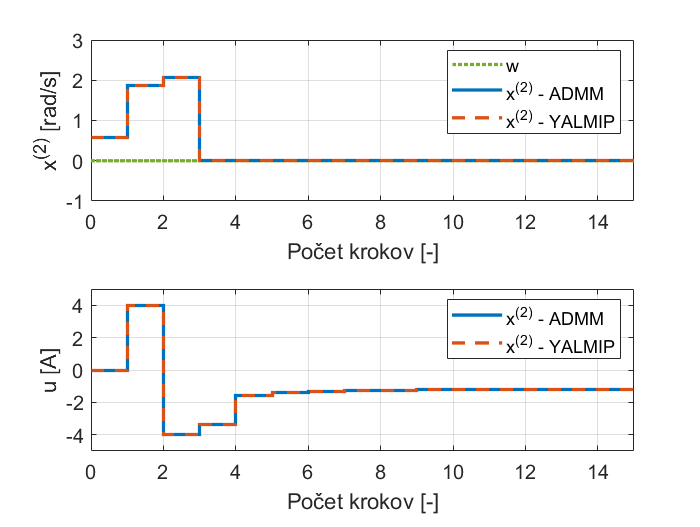
\includegraphics[width=13cm,height=10cm]{images/DC_motor/Priebeh_riadenia_a_akcne_zasahy}
	\caption{Priebeh riadenia DC motora}
	\label{fig7: PR}
\end{figure}
Ako môžeme vidieť na (Obr 3.4), v oboch prípadoch sa nám podarilo dosiahnuť žiadanú veličinu (zastavenie DC motora) s totožným priebehom riadenia. Vývoj stavu $x^{(1)}$ čo je prúd rotora nás nezaujíma a preto ho nemáme ani zobrazený.
\newpage
\begin{figure}[H]	
	\centering
	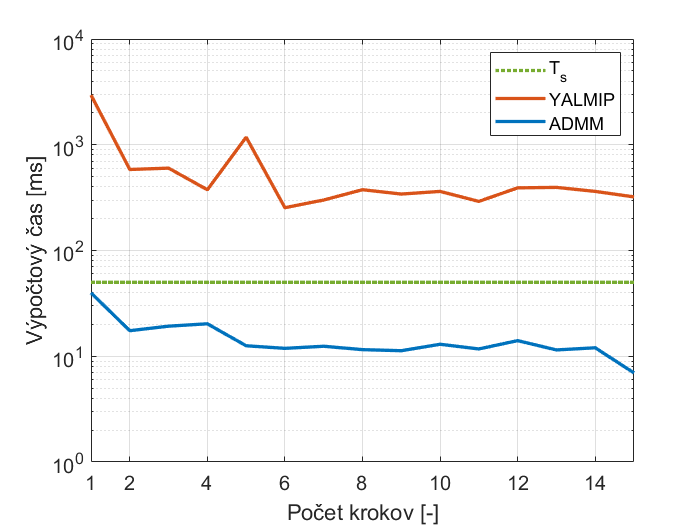
\includegraphics[width=13cm,height=10cm]{images/DC_motor/Vypoctovy_cas}
	\caption{Porovnanie výpočtovej náročnosti MPC, medzi ADMM a YALMIP}
	\label{fig9: VN}
\end{figure}
Na (Obr. 3.5) si môžeme všimnúť, že pomocou analytického riešiteľa z toolboxu YALMIP sme sa ani len nepriblížili k perióde vzorkovania DC motora, a preto nie je možné používať takýto spôsob výpočtu MPC pre riadenie daného systému. Naopak, pomocou ADMM sa nám podarilo dosiahnuť veľmi dobré výsledky. Vďaka ADMM sme mohli rozdeliť jeden optimalizačný problém na päť decentralizovaných a riešiť ich samostatne. Takéto rozdelenie zmenšilo počet iterácií v Newtonovej numerickej optimalizácii a zároveň umožnilo paralelné riešenie týchto decentralizovaných problémov. Vo výsledku vidíme, že sa nám podarilo dostatočne zrýchliť výpočet akčných zásahov a stíhame ich opakovane počítať v rámci periódy vzorkovania $T_{s} = 50ms$.